\section{Evaluation of Porting Strategies}\label{sec:evaluation-of-porting-strategies}
Following the prototype publication, various intermediate solutions were hypothesised, tested and discarded
before arriving at the current version of the Keyrtual mobile application.
This section will explore the various steps that led us to the final version,
the unsuccessful attempts and the reasons why certain choices were made.

\subsection{Depth vision}\label{subsec:depth-vision}
Nowadays, the presence of two or more photo sensors has become the standard for all smartphones, even low-end ones.
Among the sensors that can be found on smartphones there are for example
depth sensors, macro sensors, wide-angle sensors and tele sensors.

One of the first ideas, when we started thinking about porting the project to smartphones,
was to use these different sensors to derive information about the position of the hands
in the three-dimensional space of the scene, in two possible ways:
\begin{itemize}
	\item \textit{Depth sensor:} directly use the smartphone's depth sensor to obtain depth information on the
	playing fingers, to be combined with the information obtained from the RGB sensor and MediaPipe,
	just like in the first prototype.
	\item \textit{Stereo vision:} use two different camera sensors at the same time to capture two images
	of the same scene, from two slightly different points of view, and then use classic stereo
	vision algorithms to derive the depth of the hands in the scene.
\end{itemize}

At first glance, both of these methods might seem excellent for solving the problem of depth
ambiguity in single-perspective images, but unfortunately both have technical
difficulties that make them practically unusable in our use case.

\subsubsection{Depth sensor}
The depth sensor in smartphones is used, among other things, to improve focus, sharpness and to apply visual
effects on the final image, such as background blur and focus on an object in the foreground.
The idea of using this sensor to derive depth information on the hand is unfortunately
unrealistic given the low resolution and sensitivity of this type of sensor.

In our case, we need an accuracy in detecting depth in the order of a centimetre.
In fact, to detect the touch of a finger, we need to detect a small change in depth, of about 1 cm,
in the area of a single finger, about 1 cm$^2$ in size, at a distance from the sensor of about 40 cm.

This accuracy could perhaps be achieved by the sensors built in a handful of high-end smartphones, but since
one of the goals of this project is to reach as many devices as possible, this method was abandoned very early on.

\subsubsection{Stereo vision}
This method presents even greater technical difficulties than the previous one.
Firstly, as mentioned above, although smartphones are equipped with multiple camera sensors,
they all perform a different function and differ deeply in terms of size, accuracy and the type of output produced.
To use the stereo vision technique, one would need a smartphone with two identical cameras.

Moreover, the presence and positioning of these sensors on the back of the smartphone is by no means regular,
and can vary greatly from model to model.
This would be a major obstacle in using stereo vision algorithms,
which depend on the position and proximity of the sensors used.

\begin{figure}[ht]
	\captionsetup[subfigure]{labelformat=empty}
	\centering
	\begin{subfigure}{0.3\textwidth}
		\centering
		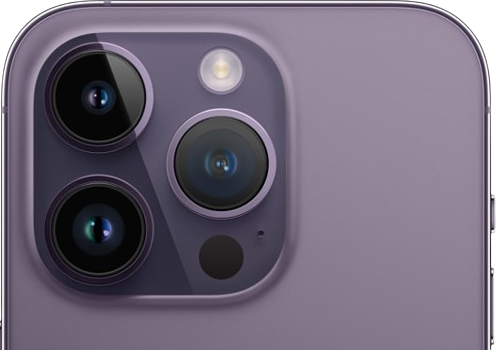
\includegraphics[width=\textwidth]{images/back-camera-iphone-14-pro}
		\caption{Iphone 14 Pro}
	\end{subfigure}
	\hfill
	\begin{subfigure}{0.3\textwidth}
		\centering
		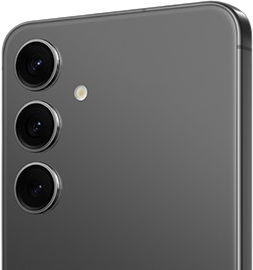
\includegraphics[width=\textwidth]{images/back-camera-galaxy-s24}
		\caption{Samsung Galaxy S24}
	\end{subfigure}
	\hfill
	\begin{subfigure}{0.3\textwidth}
		\centering
		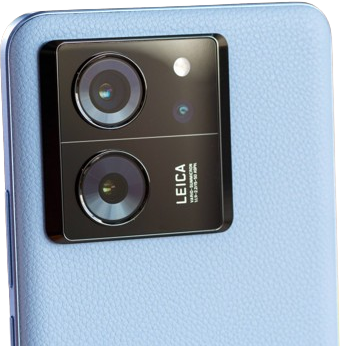
\includegraphics[width=\textwidth]{images/back-camera-redmi-13t}
		\caption{Xiaomi 13T}
	\end{subfigure}
	\caption{Different models of smartphone with different camera sensor number and position.}
	\label{fig:back-cameras}
\end{figure}

\subsubsection{Dedicated software}
We also considered the possibility of using dedicated software to calculate a depth map from an RGB image,
such as MiDaS~\cite{midas}.
Unfortunately, these models are not designed for use on mobile devices,
and require computing power that is not available on smartphones.

Although there are versions designed specifically for mobile devices,
the resulting depth maps are not precise enough for our purpose.

\subsection{MediaPipe for 3D coordinates}\label{subsec:mp-for-3d}
MediaPipe's hand detection feature not only detects hand landmarks as 2D coordinates in the image,
but also produces extra coordinates representing the position of the landmarks in 2.5D space.
In the 2.5D space, in addition to the existing $x$ and $y$ axes, a new $z$ axis is added to represent the landmark
depth with the depth at the wrist being the origin, and the smaller the value the closer the landmark is to the camera.

Among the methods hypothesised for porting the project to smartphones was to use this new coordinate to assess
whether a finger was pressing on a button, using the $z$ axis value.
This method immediately revealed a number of problems, including the fact that the $z$ coordinate,
being derived from a single RGB image, is not precise and is also very flickering.

In addition, the $z$ coordinate is not expressed in absolute reference but in reference to the landmark located in
the wrist, which makes its value variable not only according to the position of the individual landmark
but according to the position of the entire hand in relation to the wrist.

\subsection{Point of view}\label{subsec:pov}
A very important difference between the new and the old prototype is the change in the positioning of the camera.
In the first prototype we chose to use a 90\degree \ angle, which gave us a very good view of the keyboard,
precise information on the position of the hands on the plane in relation to the keys and, thanks
to the Leap Motion sensor, precise information on the distance and position of the hands in three-dimensional space.
This results in complete information on the $x_w$ and $y_w$ axes ($x$ and $y$ world axes) given by the RGB sensor,
and excellent information on the $z_w$ axis given by the Leap Motion sensor.

In the new version, in which we only have the RGB sensor, using the same positioning of the camera,
the $z_w$ axis information is totally lost.
This can be partially recovered thanks to MediaPipe, which however does not provide sufficiently precise
depth coordinates but rather inconsistent and flickering, so we could not rely solely on them.

Instead, we preferred to exploit a 45\degree \ angle of the camera in order to make the best use of the partial
information this viewpoint provides us with regarding the $z_w$ axis.
Changing the angle from 90\degree \ to 45\degree, in fact,
provides us with partial information on the $z_w$ axis that is completely absent in the top view.
The two methods are illustrated in \autoref{fig:camera-povs}.

The first method, that of the old prototype explained
in~\autoref{subsec:real-time-phase-prototype}~\nameref{subsec:real-time-phase-prototype},
gave complete information on the $x_w$ and $y_w$ axes, but no information on the $z_w$ axis.
This shortcoming, shown in \autoref{fig:camera-pov-90}, was compensated for by the use of the Leap Motion sensor,
which provided accurate depth data and allowed the system to function correctly.

However, this method is no longer usable now that we only have an RGB camera at our disposal,
and we were therefore forced to change to a different angle.
This new viewpoint has the advantage of gaining partial information about the $z_w$ axis, at the cost of a partial
loss of information about the $y_w$ axis, both of which are visible in \autoref{fig:camera-pov-45}.

The result is that the $y_w$ and $z_w$ axes are partially merged and ``compressed'', becoming part of the same
$y_s$ axis ($y$ screen axis, given by MediaPipe), while the $x_w$ axis
maintains a virtually exact correspondence with the $x_s$ axis.

\begin{figure}[ht]
	\centering
	\begin{subfigure}{0.49\textwidth}
		\centering
		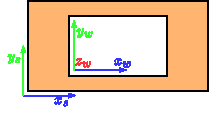
\includegraphics[width=\textwidth]{images/application/camera-pov-90}
		\caption{Camera angle at 90\degree}
		\label{fig:camera-pov-90}
	\end{subfigure}
	\hfill
	\begin{subfigure}{0.49\textwidth}
		\centering
		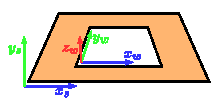
\includegraphics[width=\textwidth]{images/application/camera-pov-45}
		\caption{Camera angle at 45\degree}
		\label{fig:camera-pov-45}
	\end{subfigure}
	\caption{
		Different points of view of the camera on the paper sheet.
		The lower the angle, the more precision about axis $z_w$ but less precision about $y_w$.
	}
	\label{fig:camera-povs}
\end{figure}

The partial loss of information on the $y_w$ axis, however, is not a problem at all: it is in fact only used for
note recognition, and this only occurs when a touch is recognised, i.e.\ when the finger presses directly on the paper.
The loss of information on the $y_w$ axis, therefore, does not affect note recognition at all,
nor the functioning of the application in general.

Thanks to the presence of the frame area, during keyboard detection,
we can force the correct positioning of the smartphone, guaranteeing the success of real-time phase.
